\documentclass[11pt]{article}
\usepackage[margin=1in]{geometry}
\usepackage{amsmath,amssymb,amsthm,mathtools}
\usepackage{graphicx}
\usepackage[hidelinks]{hyperref}
\usepackage{microtype}
\usepackage{xcolor}

\newtheorem{theorem}{Theorem}
\newtheorem{lemma}[theorem]{Lemma}
\newcommand{\R}{\mathbb R}
\newcommand{\HH}{\mathcal H}
\newcommand{\dd}{\,d}
\newcommand{\supp}{\operatorname{supp}}

\title{A uniform BV--flux bound for the corrected\\
semi-discrete Brenier interface conjecture}
\author{Automated mathematics discovery run \texttt{fa\_banach\_001}\\
Lane 13, model GPT5.6}
\date{9 August 2026}

\begin{document}
\maketitle

\begin{center}
\fbox{\parbox{0.91\textwidth}{\textbf{Status.}
Candidate full solution, likely valid, subject to human review.  The theorem
proves the corrected conjecture in Remark 6.12 of the 2025 published version
of Divol--Niles-Weed--Pooladian, in its natural common-bounded-support
formulation.  The arXiv-v1 mass-ratio expression is separately shown to be
false and was removed in the published normalization.}}
\end{center}

\section{The corrected conjecture and the version issue}

Let a source probability measure have density $\rho$ on $\R^d$, and let
\[
 \mu=\sum_{j=1}^J\mu_j\delta_{y_j},\qquad \mu_j>0,
\]
be a discrete target.  The semi-discrete Brenier potential is polyhedral:
\[
 \phi(x)=\max_{1\leq j\leq J}
 \{\langle x,y_j\rangle-\psi_j\}.
\]
Its gradient is $y_j$ on the corresponding Laguerre cell $L_j$.
For $x\in L_i$, the source defines
\[
 \Delta_{ij}(x)=2\bigl(\langle x,y_i-y_j\rangle
 -\psi_i+\psi_j\bigr),
 \qquad H_{ij}(t)=\{x\in L_i:\Delta_{ij}(x)=t\},
\]
and
\[
 h_{ij}(t)=\int_{H_{ij}(t)}\rho(x)\dd\HH^{d-1}(x).
\]

The arXiv-v1 remark conjectured uniform boundedness of
\[
 Q_{\mathrm{v1}}(\mu)=
 \sum_{i,j}\|y_i-y_j\|h_{ij}(0)
 \log(1+\mu_j/\mu_i).
 \tag{1}
\]
This cannot be the correct coefficient.  For the uniform source on $[0,1]$,
target atoms $y_1=0,y_2=1$, and masses
$(\mu_1,\mu_2)=(\delta,1-\delta)$, the cells meet at $x=\delta$, and
$h_{12}(0)=h_{21}(0)=1$.  Hence
\[
 Q_{\mathrm{v1}}(\mu)
 =-\log\bigl(\delta(1-\delta)\bigr)\longrightarrow\infty
 \qquad(\delta\downarrow0).
 \tag{2}
\]

The published normalization absorbs the masses into the entropic dual
potential,
$(\widetilde\psi_\varepsilon)_j=(\psi_\varepsilon)_j
-\varepsilon\log\mu_j$.  The coefficient in the revised Remark 6.12 is
instead
\[
 Q(\mu)=\log 2\sum_{i,j}\|y_i-y_j\|h_{ij}(0),
 \tag{3}
\]
and the authors conjecture that it is uniformly bounded over discrete
measures.

\begin{figure}[h]
  \centering
  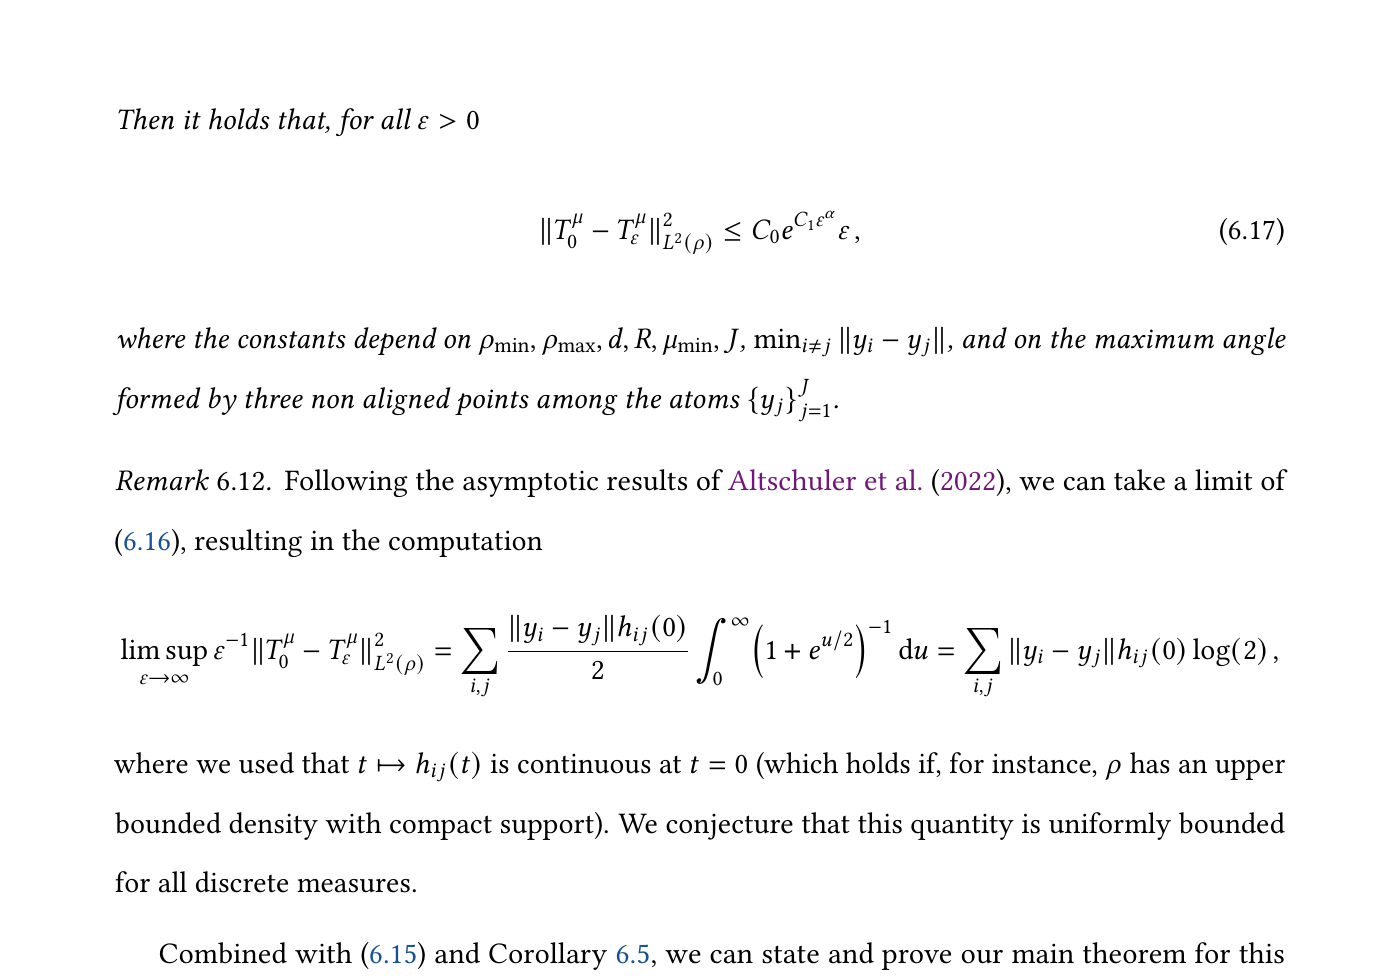
\includegraphics[width=0.98\textwidth]{figures/source_conjecture_revised.png}
  \caption{The corrected coefficient and conjecture, reproduced in
  Remark 6.12 of the author's thesis chapter based on the 2025 article.}
\end{figure}

\section{Uniform interface theorem}

\begin{theorem}\label{thm:main}
Suppose $0\leq\rho\leq M$, with
$\supp\rho\subseteq B(0,R_x)\subset\R^d$, and suppose all target atoms
satisfy $y_j\in B(0,R_y)$.  Then
\[
 Q(\mu)\leq
 2d\omega_d M R_yR_x^{d-1}\log 2,
 \tag{4}
\]
where $\omega_d$ is the volume of the Euclidean unit ball.  The bound is
independent of $J$, of the masses $\mu_j$, of the minimum atom separation,
and of the combinatorics of the Laguerre diagram.

In particular, if source and target supports lie in the common ball
$B(0,R)$, then
\[
 Q(\mu)\leq 2d\omega_d M R^d\log 2.
 \tag{5}
\]
\end{theorem}

\begin{proof}
Repeated target atoms may be merged, so assume the $y_j$ are distinct.
The function $\phi$ is convex and globally $R_y$-Lipschitz.  Its gradient
$T=\nabla\phi$ is a piecewise-constant BV map whose values on the interiors
of the Laguerre cells are the $y_j$.

Let $F_{ij}$ be the relative interior of a common codimension-one facet of
$L_i$ and $L_j$.  Direct the unit normal from $L_i$ to $L_j$.  Since
$L_i$ is the side on which
\(\langle x,y_i-y_j\rangle-\psi_i+\psi_j\geq0\), this normal is
\[
 \nu_{ij}=\frac{y_j-y_i}{\|y_j-y_i\|}.
\]
The BV jump formula therefore gives
\[
 D(\nabla\phi)\mathbin{\vrule height 1.4ex depth -0.2ex width 0.07ex
 \vrule height 0.07ex depth -0.0ex width 0.7ex}_{F_{ij}}
 =(y_j-y_i)\otimes\nu_{ij}\,
 \HH^{d-1}\mathbin{\vrule height 1.4ex depth -0.2ex width 0.07ex
 \vrule height 0.07ex depth -0.0ex width 0.7ex}_{F_{ij}}.
\]
Taking the trace shows that the distributional Laplacian of $\phi$ has
facet density
\[
 \Delta\phi\mathbin{\vrule height 1.4ex depth -0.2ex width 0.07ex
 \vrule height 0.07ex depth -0.0ex width 0.7ex}_{F_{ij}}
 =\|y_i-y_j\|\,
 \HH^{d-1}\mathbin{\vrule height 1.4ex depth -0.2ex width 0.07ex
 \vrule height 0.07ex depth -0.0ex width 0.7ex}_{F_{ij}}.
 \tag{6}
\]
Lower-dimensional multiple-tie sets carry no $\HH^{d-1}$ mass.  Inactive
affine pieces can be discarded.  Thus (6) accounts for the whole Laplacian
measure of the polyhedral convex function.

At $t=0$, $H_{ij}(0)$ is precisely the trace of the common facet on $L_i$.
The ordered sum counts every facet twice.  Therefore, for any $r>R_x$,
\[
\begin{aligned}
 \sum_{i,j}\|y_i-y_j\|h_{ij}(0)
 &=2\sum_{i<j}\|y_i-y_j\|
   \int_{F_{ij}}\rho\dd\HH^{d-1}\\
 &\leq 2M\,\Delta\phi(B(0,r)).
\end{aligned}
\tag{7}
\]

It remains only to bound the total Laplacian mass.  Let
$\phi_\eta=\phi*\zeta_\eta$ be a standard mollification.  Convexity and the
gradient bound are preserved:
$\|\nabla\phi_\eta\|\leq R_y$.  By the divergence theorem,
\[
\begin{aligned}
 \Delta\phi_\eta(B(0,r))
 &=\int_{\partial B(0,r)}
   \nabla\phi_\eta\cdot n\dd\HH^{d-1}\\
 &\leq R_y\HH^{d-1}(\partial B(0,r))
 =d\omega_dR_y r^{d-1}.
\end{aligned}
\tag{8}
\]
The nonnegative measures $\Delta\phi_\eta$ converge weakly to
$\Delta\phi$.  For all but countably many radii the boundary has zero
$\Delta\phi$-mass, so (8) passes to the limit.  Choosing such radii
$r\downarrow R_x$ and using (7) yields
\[
 \sum_{i,j}\|y_i-y_j\|h_{ij}(0)
 \leq2d\omega_dMR_yR_x^{d-1}.
\]
Multiplication by $\log2$ proves (4), and (5) follows by taking
$R_x=R_y=R$.
\end{proof}

\section{Interpretation and checks}

The proof identifies the conjectured interface sum with twice a weighted
part of the trace measure of $D^2\phi$.  Convexity makes this Hessian measure
positive, while the bound on the slopes of $\phi$ converts its total mass
into boundary flux.  This is why neither small target masses nor complicated
Laguerre diagrams cause divergence in the corrected expression.

In dimension one, the identity reduces to the elementary statement that the
sum of successive jumps of a monotone step function is its total variation.
For the two-atom example used in (2), the corrected quantity is always
$2\log2$, independently of $\delta$.

The common target-support bound is necessary.  If ``all discrete measures''
is interpreted literally with no common bound on the atom locations, scaling
two target atoms scales $Q$ linearly.  Theorem~\ref{thm:main} resolves the
fixed-ball formulation used in the stability results of the source paper.

\section{Novelty audit and reviewer focus}

The run's registry, solution, attempt, and proof-gap indexes were searched
for arXiv:2404.02855, the exact paper title, the corrected expression,
Laguerre-interface sums, BV variation, and Brenier-potential flux; no
duplicate was found.  Bounded literature searches on 9 August 2026 used the
exact conjecture sentence and formula and checked later work on semi-discrete
entropic maps.  The corrected conjecture remains present in the published
article's thesis reproduction, and no later resolution was located.

The main reviewer checks are the factor of two in (7), the treatment of
degenerate multiple ties, and the intended common-support interpretation of
``uniformly bounded.''  The first follows because the source sums ordered
pairs; the second is the standard BV jump decomposition after inactive
pieces are removed.  Novelty confidence is moderate because the underlying
BV and divergence facts are classical, though their application here seems
unrecorded.

\begin{thebibliography}{9}
\bibitem{DNWP}
V. Divol, J. Niles-Weed, and A.-A. Pooladian,
\emph{Tight Stability Bounds for Entropic Brenier Maps},
International Mathematics Research Notices, 2025(7), rnaf078 (2025),
\href{https://doi.org/10.1093/imrn/rnaf078}{doi:10.1093/imrn/rnaf078};
arXiv:\href{https://arxiv.org/abs/2404.02855}{2404.02855}.

\bibitem{PooladianThesis}
A.-A. Pooladian,
\emph{Statistical and Algorithmic Perspectives on Optimal Transport},
doctoral thesis, 2025, Chapter 6 and Appendix E.5.

\bibitem{AFP}
L. Ambrosio, N. Fusco, and D. Pallara,
\emph{Functions of Bounded Variation and Free Discontinuity Problems},
Oxford University Press, 2000.
\end{thebibliography}

\end{document}
